%_______________________________________________________________________________
%_______________________________________________________________________________
%_______________________________________________________________________________

\ifthenelse{\boolean{cms@external}}{\providecommand{\suppMaterial}{the supplemental material [URL will be inserted by publisher]}}{\providecommand{\suppMaterial}{Appendix~\ref{app:suppMat}}}

\newcommand{\njet}{\ensuremath{n_{\text{jet}}}\xspace}
\newcommand{\nb}{\ensuremath{n_{\text{b}}}\xspace}
\newcommand{\scalht}{\ensuremath{H_{\text{T}}}\xspace}
\newcommand{\mht}{\ensuremath{H_{\text{T}}^{\text{miss}}}\xspace}

\title{Search for natural and split supersymmetric scenarios in pp
  collisions at $\sqrt{s} = 13\TeV$ in all-jet final
  states\texorpdfstring{ \\[1cm] ---Supplemental Material---}{: Supplemental Material}}

\author[cern]{The CMS Collaboration}
\address[cern]{CERN} 

\date{\today}

\abstract{}

\hypersetup{
  pdfauthor={Robert Bainbridge, Eshwen Bhal, Shane Breeze, Oliver
    Buchmueller, Stefano Casasso, Matthew Citron, Adam Elwood, Henning
    Flaecher, Aran Garcia-Bellido, Ben Krikler, Christian Laner, Kin
    Ho Lo, Sarah Alam Malik, Bjoern Penning, Tai Sakuma, Dominic
    Smith, Alex Tapper},
  pdftitle={Search for natural and split supersymmetric scenarios in pp
  collisions at 13 TeV in all-jet final states},
  pdfsubject={CMS, supersymmetry, AlphaT},
  pdfkeywords={Supersymmetry, split, natural, long-lived gluinos, dark matter}
}

%\cmsNoteHeader{SUS-16-038}
\maketitle

%\begin{figure}
%\centering
%\includegraphics[width=0.48\textwidth, trim=10 0 60 10, clip=true]{}
%\caption{}
%\end{figure}

%\begin{table}
%\topcaption{} 
%\centering
%\end{table}

\clearpage
\begin{figure}
    \begin{center}
        \subfigure[T1qqqq]{
            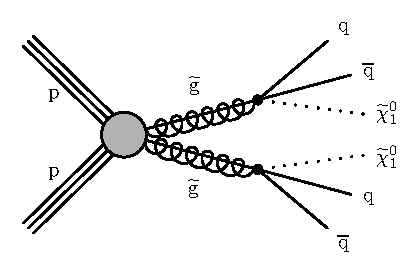
\includegraphics[width=0.3\textwidth]{Supplementary/T1qqqq_feyn_aux}
            \label{fig:T1qqqq_feyn}
        }~~
        \subfigure[T2qq]{
            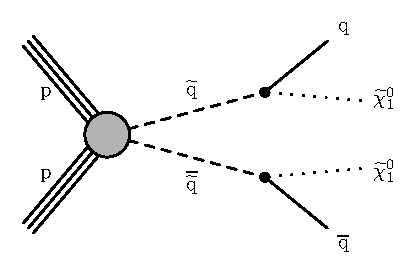
\includegraphics[width=0.3\textwidth]{Supplementary/T2qq_feyn_aux}
            \label{fig:T2qq_feyn}
        }~~
        \caption{
            Graphical representation of the production and decay of
            supersymmetric particles in ``light-flavour models'', i.e. with
            gluinos/squarks decaying to light quarks.
        }
        \label{fig:simplified-models-feyn-light}
    \end{center}
\end{figure}

\begin{figure}[h!]
    \begin{center}
        \subfigure[T1bbbb]{
            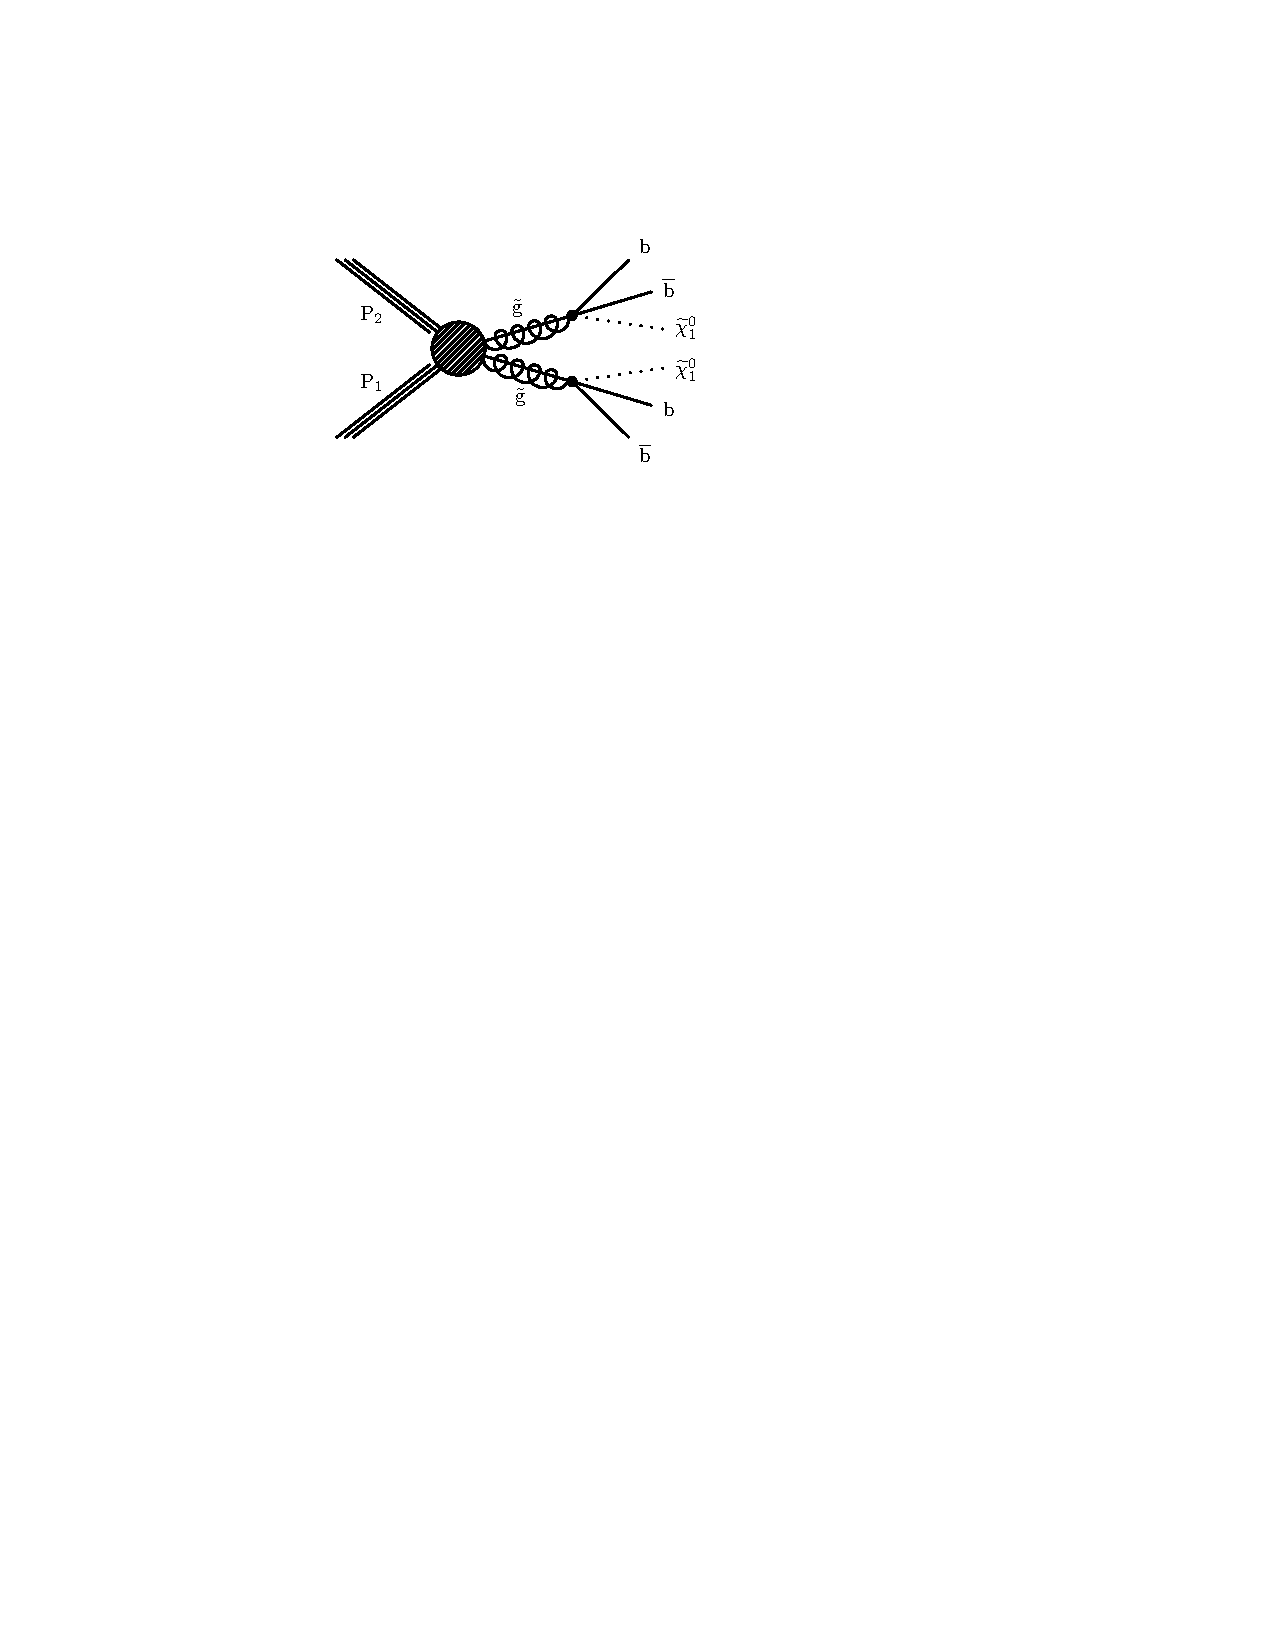
\includegraphics[width=0.3\textwidth]{Supplementary/T1bbbb_feyn_aux}
            \label{fig:T1bbbb_feyn}
        }~~
        \subfigure[T1tttt]{
            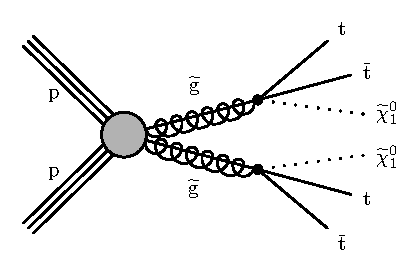
\includegraphics[width=0.3\textwidth]{Supplementary/T1tttt_feyn_aux}
            \label{fig:T1tttt_feyn}
        }~~
        \caption{
            Graphical representation of the production and decay of
            supersymmetric particles in gluino models with decoupled third
            generation squarks.
        }
        \label{fig:simplified-models-feyn-gluino}
    \end{center}
\end{figure}

\begin{figure}[h!]
    \begin{center}
        \subfigure[T2bb]{
            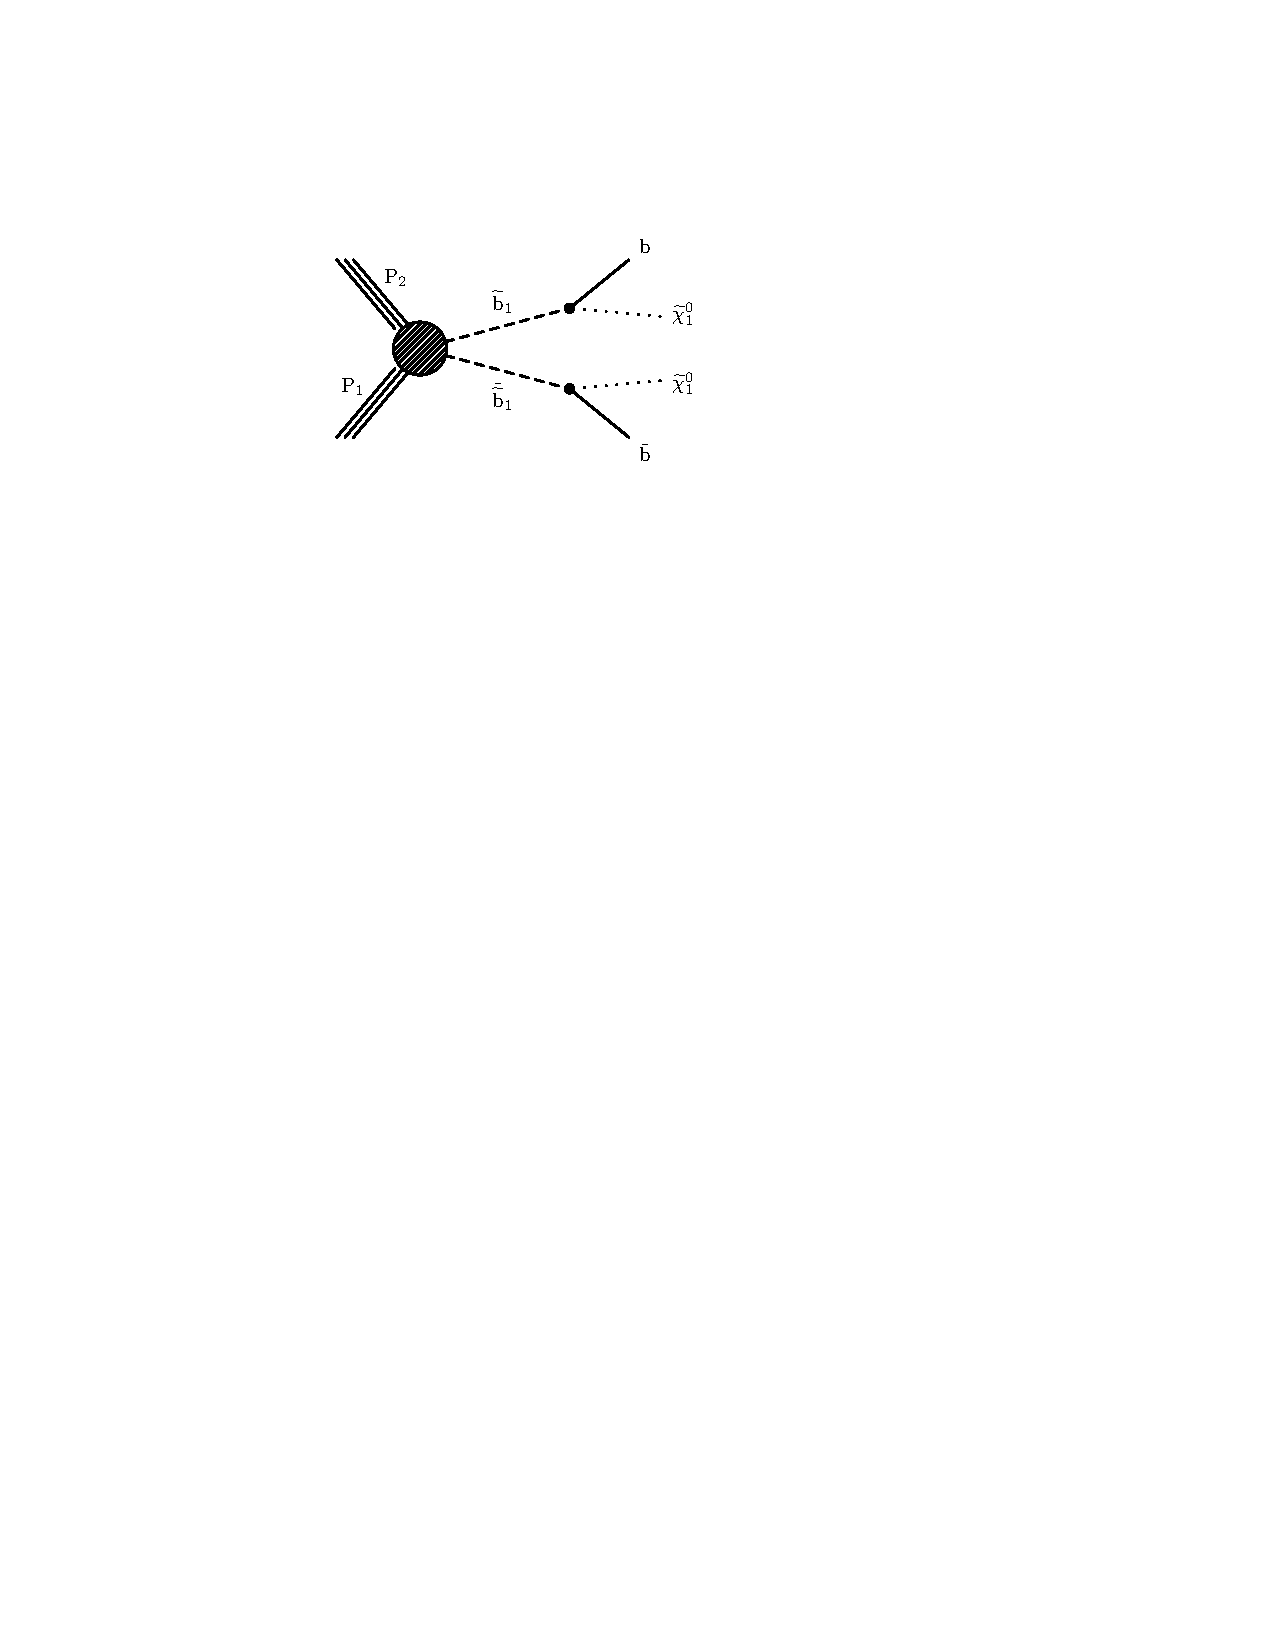
\includegraphics[width=0.3\textwidth]{Supplementary/T2bb_feyn_aux}
            \label{fig:T2bb_feyn}
        }~~
        \subfigure[T2tt]{
            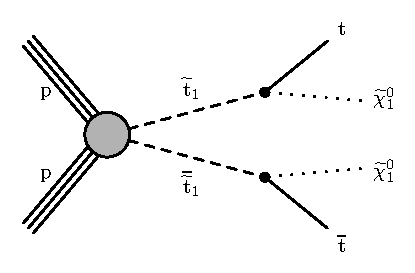
\includegraphics[width=0.3\textwidth]{Supplementary/T2tt_feyn_aux}
            \label{fig:T2tt_feyn}
        }~~
        \subfigure[T2cc]{
            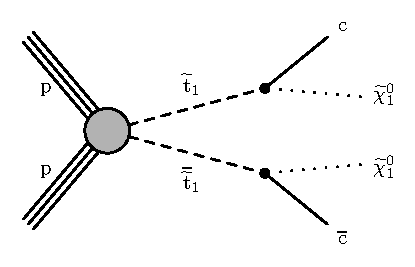
\includegraphics[width=0.3\textwidth]{Supplementary/T2cc_feyn_aux}
            \label{fig:T2cc_feyn}
        }~~
        \caption{
            Graphical representation of the production and decay of
            supersymmetric particles in models with the production of third
            generation squarks (stops and sbottomes).
        }
        \label{fig:simplified-models-feyn-3rdGen}
    \end{center}
\end{figure}

\clearpage
